\documentclass[conference]{IEEEtran}
\IEEEoverridecommandlockouts

\usepackage{cite}
\usepackage{amsmath,amssymb,amsfonts}
\usepackage{algorithmic}
\usepackage{graphicx}
\usepackage{textcomp}
\usepackage{xcolor}
\usepackage{tikz}

\usetikzlibrary{arrows.meta, positioning, shapes.geometric}

\begin{document}

\title{ML-Based Task Assignment and Deadline Prediction for Agile Project Management with Automated Workflow Integration}

\author{
\IEEEauthorblockN{Muhammad Risyad Himawan Putra}
\IEEEauthorblockA{
Department of Informatics\\
Institut Teknologi Sepuluh Nopember\\
Surabaya, Indonesia\\
5025231205@student.its.ac.id
}
\and
\IEEEauthorblockN{Riyanarto Sarno}
\IEEEauthorblockA{
Department of Informatics\\
Institut Teknologi Sepuluh Nopember\\
Surabaya, Indonesia\\
riyanarto@its.ac.id
}
\and
\IEEEauthorblockN{Kurnia Cahya Febryanto}
\IEEEauthorblockA{
Department of Informatics\\
Institut Teknologi Sepuluh Nopember\\
Surabaya, Indonesia\\
6025241065@student.its.ac.id
}
\and
\IEEEauthorblockN{Kelly Rossa Sungkono}
\IEEEauthorblockA{
Department of Informatics\\
Institut Teknologi Sepuluh Nopember (ITS)\\
Surabaya, Indonesia\\
kelsungkono@gmail.com
}
\and
\IEEEauthorblockN{Asra Al Fauzi}
\IEEEauthorblockA{
Neurosurgery\\
Universitas Airlangga\\
Surabaya, Indonesia\\
fao\_int@fk.unair.ac.id
}
\and
\IEEEauthorblockN{Setiawan Hadi}
\IEEEauthorblockA{
Computer Science\\
Universitas Padjadjaran\\
Bandung, Indonesia\\
setiawanhadi@unpad.ac.id
}
}



\maketitle

\begin{abstract}
Agile and Scrum teams often face inconsistent task assignment, uncertain deadline estimation, and high manual overhead during sprint execution. This study investigates the feasibility of embedding machine learning predictions into an automated Agile workflow to support assignee recommendation and deadline estimation. Using a subset of the Aurora project data (N=825), an XGBoost-based multi-class classifier is trained for assignee recommendation, achieving 77.58\% Top-1 accuracy and 95.15\% Top-3 accuracy on an unseen hold-out set. For deadline prediction, a Combined Aurora and Mesos dataset (N=2,607, filtered to 933 active sprint tasks) is utilized to train a robust Random Forest regressor. The selected deadline model achieves a Mean Absolute Error (MAE) of 6.62 days and a Mean Absolute Percentage Error (MAPE) of 38.5\%, successfully outperforming a grouped median baseline (MAE 7.01 days) despite the high variance inherent in issue resolution times. The models are deployed as REST endpoints and integrated into an n8n-orchestrated workflow, enabling automated field updates and periodic re-evaluation during active sprints. Results demonstrate the operational feasibility of ML-driven workflow automation while highlighting the challenge of precise time estimation in heterogeneous Agile environments.
\end{abstract}

\begin{IEEEkeywords}
Agile Software Development, Task Assignment, Deadline Prediction, Machine Learning, Workflow Automation
\end{IEEEkeywords}

\begin{table*}[t]
\caption{Gap Analysis of Recent Work and the Positioning of This Study}
\centering
\renewcommand{\arraystretch}{1.2}
\begin{tabular}{p{3.0cm} p{4.2cm} p{4.5cm} p{5.0cm}}
\hline
\textbf{Study} & \textbf{Approach} & \textbf{Limitation} & \textbf{Gap Addressed by This Work} \\
\hline
Shamim et al. \cite{shamim2025_costreview} &
Review of AI for cost/effort estimation &
Model-centric; limited discussion on operational workflow embedding &
Deployable ML services integrated into workflow engine for real-time execution \\
Sousa et al. \cite{sousa2023_task_effort} &
ML for task effort/duration estimation &
Standalone predictor; not integrated into automation loop &
Predictions trigger automated updates and periodic re-evaluation during sprint \\
Prinz et al. \cite{prinz2021_lowcode_slr} &
Low-code platform literature review &
Automation often rule-based; brittle with evolving contexts &
ML-driven predictions adapt workflows beyond static rules \\
Yasmin et al. \cite{yasmin2024_airflow_wac} &
Workflows-as-code challenges &
Focus on orchestration challenges; not project-ticket automation &
Applies orchestration concepts to Agile tickets with ML decision support \\
P\'erez Castillo et al. \cite{perezcastillo2024_sprint_velocity} &
Sprint progress/velocity evaluation &
Sprint analytics; limited automation into issue operations &
Operationalizes sprint monitoring via scheduled re-check and automated updates \\
Diamantopoulos et al. \cite{diamantopoulos2023_issue_assignment} &
Automated issue assignment &
Assignment recommendation without end-to-end workflow enforcement &
End-to-end pipeline: prediction $\rightarrow$ update fields $\rightarrow$ notify $\rightarrow$ re-check \\
\textbf{Proposed Method} &
\textbf{Supervised ML integrated into n8n workflow orchestration} &
\textbf{Focus on operational feasibility; limited by available metadata} &
\textbf{Empirical evaluation and workflow-aware integration enabling real-time updates} \\
\hline
\end{tabular}
\label{table:gap}
\end{table*}


% =========================================================
\section{Introduction}
Agile and Scrum have become dominant approaches for managing modern software projects due to their iterative delivery and rapid feedback cycles. Empirical evidence suggests Scrum is widely practiced, with large-scale reviews indicating that Scrum or hybrid variants are used by the majority of organizations \cite{verwijs2023_scrum}. Comparisons also indicate that agile approaches can improve stakeholder success compared to purely traditional methods \cite{gemino2021_project_success}. Despite this adoption, teams frequently face operational challenges such as sprint delays and workload imbalance. These issues are intensified by high coordination demands; evidence from analytics on IT professionals shows that working hours can increase by approximately 30\% and measured productivity can decline in the 8--19\% range under higher coordination friction \cite{gibbs2023_wfh_productivity}. Furthermore, role clarity is critical for sustainability, as clearer role perceptions in agile teams are associated with reduced work exhaustion \cite{venkatesh2020_work_exhaustion}. In practice, however, project decision-making regarding task assignment and deadlines is often handled manually, amplifying delays and inconsistency under sprint pressure.

A key limitation of current project management automation is its predominantly rule-based nature. Research on low-code platforms indicates that while they accelerate automation, the resulting workflows rely on static trigger-action logic that becomes brittle under evolving project contexts \cite{prinz2021_lowcode_slr, zhao2021_trigger_action}. In parallel, machine learning has been effectively applied to specific tasks such as issue assignment \cite{diamantopoulos2023_issue_assignment} and effort or duration estimation \cite{sousa2023_task_effort}. However, a significant gap remains in the operationalization of these models: existing ML approaches are typically evaluated in an offline setting \cite{mahdi2021_spm_slr, cabral2023_ensemble_effort} and lack integration with execution pipelines \cite{yasmin2024_airflow_wac}. Consequently, prediction outputs rarely trigger automated actions or continuous re-evaluation during active sprints, limiting their practical utility for real-time decision support.

To address this gap, this study proposes an integrated architecture that operationalizes ML predictions directly inside an n8n-orchestrated Agile workflow via RESTful services. Specifically, we evaluate the predictive capability of Jira-like issue metadata for assignee recommendation and deadline estimation using supervised learning models trained on historical project data. Furthermore, we demonstrate the feasibility of embedding these predictions into automated workflow actions, such as field updates and status transitions, and present a mechanism for periodic re-evaluation to maintain prediction relevance for active issues throughout the sprint lifecycle.

% =========================================================
\section{Related Work}
% =========================================================

This section reviews machine learning applications in software project management, workflow automation, and agile prediction, summarized in Table~\ref{table:gap}.

% -------------------------------------------------------------
\subsection{Machine Learning for Software Project Management}
% -------------------------------------------------------------
Machine learning (ML) has been widely applied to support project decisions, particularly in cost, effort, and risk estimation. Systematic reviews indicate that supervised and ensemble approaches generally outperform traditional statistical baselines, though many studies remain offline and context-dependent \cite{shamim2025_costreview, mahdi2021_spm_slr}. Beyond high-level effort estimation, recent work has explored task-level duration prediction using issue metadata, demonstrating that lightweight features can yield reliable estimates suitable for tool integration \cite{sousa2023_task_effort}. However, these approaches primarily focus on prediction accuracy rather than deployment within live execution environments.

% -------------------------------------------------------------
\subsection{Workflow Automation in Software Development}
% -------------------------------------------------------------
Workflow automation platforms orchestrate actions across tools like Jira and GitHub. Research on low-code automation shows these platforms reduce development effort but often rely on static, rule-based logic that becomes brittle under evolving project contexts \cite{prinz2021_lowcode_slr}. While "workflows-as-code" approaches (e.g., Airflow) offer greater reproducibility, they present significant configuration challenges for developers \cite{yasmin2024_airflow_wac}. Furthermore, current automation research focuses heavily on authoring assistance or rule synthesis \cite{gupta2023_action_suggestions, zhao2021_trigger_action}, rather than embedding predictive intelligence directly into the operational loop.

% -------------------------------------------------------------
\subsection{Agile Sprint Prediction and Planning}
% -------------------------------------------------------------
Sprint planning relies on accurate forecasting of velocity and progress. Prior studies have utilized ML to evaluate sprint progress based on historical artifacts \cite{perezcastillo2024_sprint_velocity} and explored representation learning (e.g., Sprint2Vec) to capture sprint dynamics \cite{choetkiertikul2025_sprint2vec}. Regression and NLP-enhanced models have also been applied to story-point estimation \cite{ramessur2021_sprint_effort, yalciner2024_storypoint_sbert}. However, these models typically operate as standalone predictors for planning sessions, rather than as real-time services that continuously update field data during active sprints.

% -------------------------------------------------------------
\subsection{Task Assignment and Resource Allocation}
% -------------------------------------------------------------
Automated task assignment has been approached via developer recommendation and topic modeling on issue tracking data \cite{diamantopoulos2023_issue_assignment}. Deep learning and multimodal ensembles have further improved assignment quality by modeling developer activity \cite{guo2020_bug_triage, zhang2023_susrec}. Despite these advances, integration is often limited to recommendation lists, lacking end-to-end enforcement where the system automatically assigns and notifies developers within the workflow engine.

% -------------------------------------------------------------
\subsection{Research Gap Analysis}
% -------------------------------------------------------------
As summarized in Table~\ref{table:gap}, three consistent gaps emerge from the literature. First, most ML studies for project management remain offline and do not operationalize predictions within active workflows. Second, automation research predominantly emphasizes rule-based execution rather than data-driven decision updates. Third, task assignment and deadline estimation are typically treated as isolated problems. This work addresses these gaps by embedding supervised ML models into an n8n-orchestrated workflow that supports real-time field updates and periodic re-evaluation.

% =========================================================
\section{Proposed Method}
% =========================================================

Fig.~\ref{fig:systemflow} summarizes the end-to-end architecture: dataset preparation and training (offline), deployment as REST services, and n8n-based orchestration connected to Jira/GitHub for sprint-time automation.

\begin{figure*}[t]
\centering
    \centering
    
\includegraphics[width=0.5\linewidth]{figures/system_flow.png}
\caption{System architecture: offline training, REST deployment, and n8n orchestration for sprint-time automation.}
\label{fig:systemflow}
\end{figure*}

% ---------------------------------------------------------
\subsection{Dataset and Feature Representation}
% ---------------------------------------------------------

The dataset is the AgileScrumSprintVelocityDataSet \cite{koralage2023_velocity}, which provides Jira-like issue metadata and sprint attributes across multiple open-source projects. The assignee model is trained on the Aurora subset (complete assignee labels), while the deadline model is trained on a filtered sprint-level subset for completion-time estimation.

For assignee prediction, each issue is encoded as a feature vector combining:
\begin{itemize}
    \item structured metadata (e.g., story points, priority, sprint attributes),
    \item categorical fields (one-hot: issue type, status, project),
    \item text content (TF--IDF on summary+description, max\_features=500).
\end{itemize}
Missing values are handled via simple imputation and categorical ``Unknown'' mapping.

For deadline prediction, we use compact numeric features:
\textit{storypoint}, \textit{points\_per\_issue}, and \textit{complexity}. The complexity proxy is:
\begin{equation}
\mathrm{complexity} = \mathrm{storypoint}\cdot(4-\mathrm{priorityid}).
\end{equation}
To reduce extreme-outlier distortion, completion times are filtered to the 7--35 day range, producing 38 clean sprint records. Evaluation uses an 80/20 hold-out split by sprint (30 train, 8 test) with seed 42.

% ---------------------------------------------------------
\subsection{Assignee Recommendation Model}
% ---------------------------------------------------------

Assignee recommendation is formulated as multi-class classification over $K$ developers. XGBoost learns an additive ensemble of trees; predicted class probabilities are:
\begin{equation}
\hat{\mathbf{p}}_i = \mathrm{softmax}\Big(\sum_{t=1}^{T} f_t(\mathbf{x}_i)\Big),
\label{eq:xgb_pred}
\end{equation}
and the objective includes multiclass log-loss and tree regularization:
\begin{equation}
\mathcal{L} = \sum_{i=1}^{N}\ell\big(y_i,\hat{\mathbf{p}}_i\big) + \sum_{t=1}^{T}\Omega(f_t).
\label{eq:xgb_obj}
\end{equation}
Top-$k$ accuracy is reported to reflect recommendation usage. Class imbalance is addressed by oversampling applied \emph{only} to training folds/partitions (never to validation/test).

% ---------------------------------------------------------
\subsection{Deadline Prediction Model}
% ---------------------------------------------------------

Deadline estimation is formulated as regression of completion duration (days) using compact features available at or near issue creation time. The final reported evaluation corresponds to the fixed 80/20 split (seed 42) on 38 sprint records. The goal is low absolute error for practical due-date suggestion; variance explanation is secondary because many latent factors (scope changes, review delays, interruptions) are not observable at prediction time.

% ---------------------------------------------------------
\subsection{Deployment and Workflow Integration}
% ---------------------------------------------------------

Models are deployed as Flask-based REST endpoints and integrated into an n8n workflow:
\begin{itemize}
    \item \texttt{/predict/all}: returns top-$k$ assignee recommendations and predicted duration (days).
\end{itemize}
n8n performs scheduled re-evaluation (bi-daily) to detect incomplete or returned issues and applies field updates in Jira. Subtasks inherit key fields from parent issues to preserve ownership consistency:
\begin{equation}
\mathrm{assignee}(s)\leftarrow \mathrm{assignee}(p),\quad
\mathrm{due}(s)\leftarrow \mathrm{due}(p),
\label{eq:inherit_rule}
\end{equation}
where $p$ is a parent issue and $s$ is its subtask. PR events from GitHub trigger transitions to review/testing, notify reviewers, and return failed items with updated description cues and revised due dates.

\begin{figure*}[t]
\centering
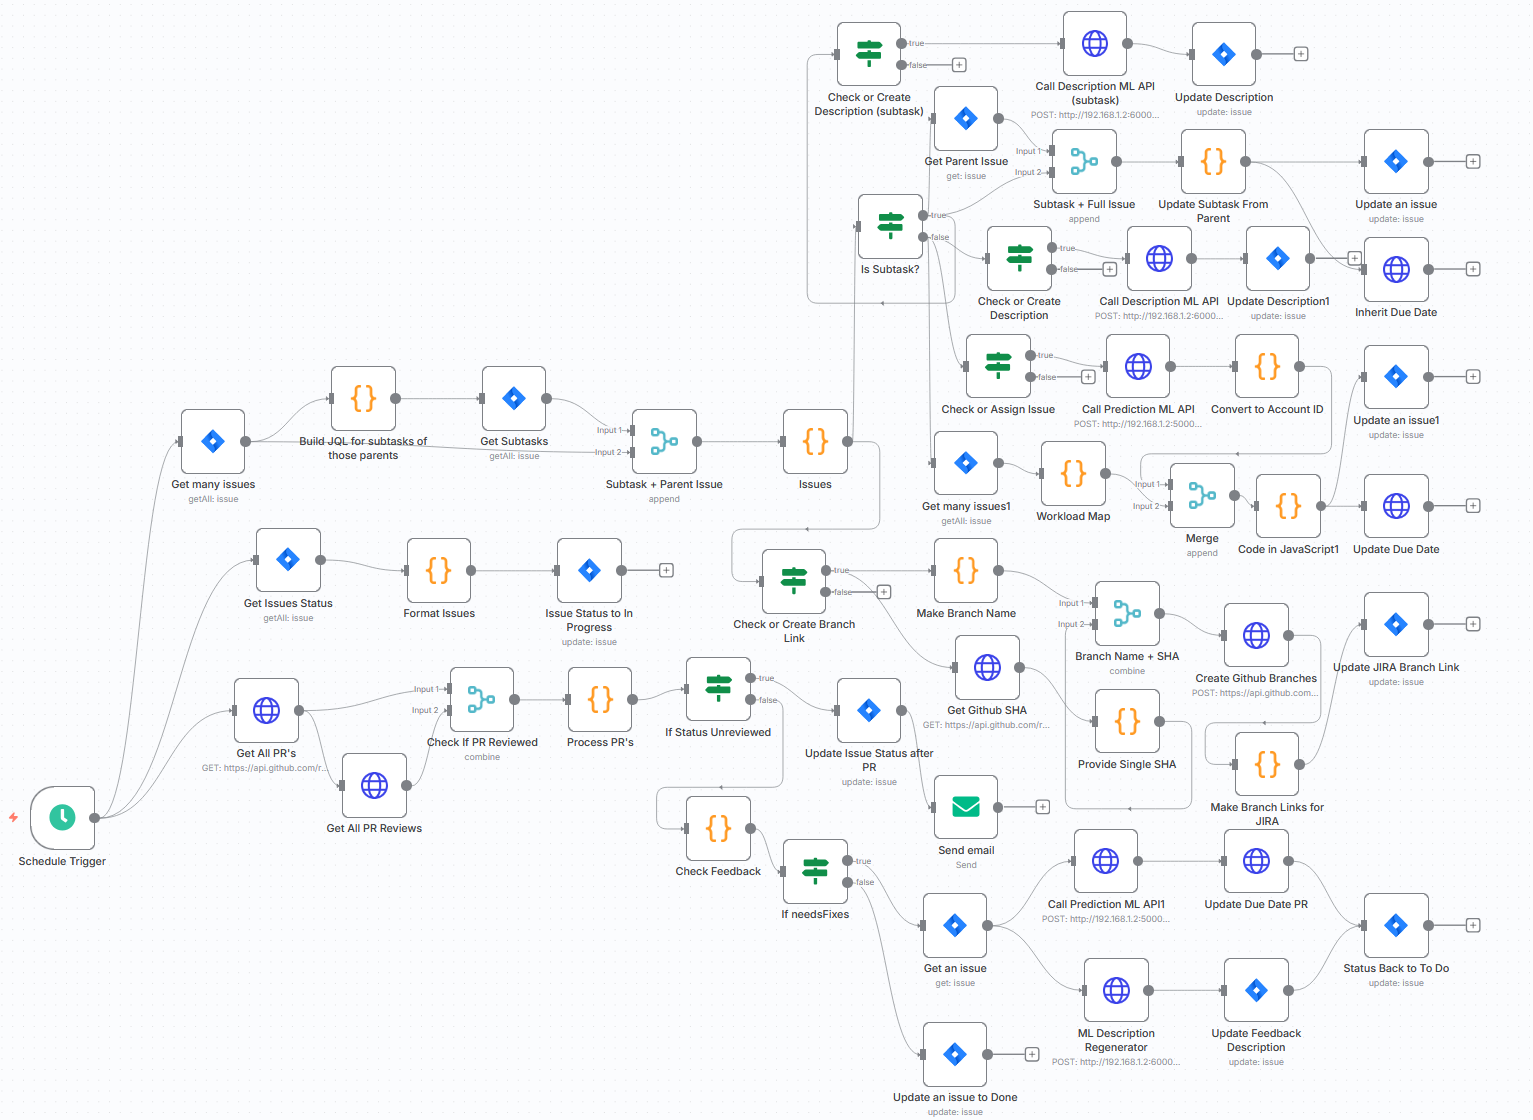
\includegraphics[width=\textwidth]{figures/n8n_flow.png}
\caption{n8n workflow for scheduled re-checks, prediction calls, Jira updates, and PR-driven transitions.}
\label{fig:n8nflow}
\end{figure*}

% =========================================================
\section{Results and Discussion}
% =========================================================

% ---------------------------------------------------------
\subsection{Experimental Setup}
% ---------------------------------------------------------

Experiments were executed on a local workstation: AMD Ryzen 9 5900HS, NVIDIA RTX 3060 Laptop (6GB), 16GB RAM, Windows 10, Python 3.11.9, scikit-learn 1.6.1, xgboost 2.1.3, flask 3.1.0.

For assignee recommendation, we report: (i) 5-fold stratified cross-validation (oversampling applied only within training folds), and (ii) an unseen 20\% hold-out test split (165 issues) to simulate deployment. For deadline prediction, evaluation is sprint-level hold-out (30 train sprints, 8 test sprints), seed 42, filtered to 7--35 days (38 records).

% ---------------------------------------------------------
\subsection{Assignee Recommendation Performance}
% ---------------------------------------------------------

Table~\ref{tab:assignee_cv} reports cross-validation accuracy and confidence intervals. NLP-enhanced models substantially outperform the dummy baseline.

\begin{table}[t]
\centering
\caption{Assignee prediction (5-fold stratified CV, oversampling only in training folds).}
\renewcommand{\arraystretch}{1.08}
\begin{tabular}{l c c}
\hline
\textbf{Model} & \textbf{Mean Acc.} & \textbf{95\% CI} \\
\hline
Dummy (Baseline) & 0.1250 & [0.1042, 0.1458] \\
Random Forest (NLP) & 0.7839 & [0.7156, 0.8522] \\
XGBoost (NLP) & 0.7851 & [0.7273, 0.8429] \\
SVM (NLP) & 0.7766 & [0.7164, 0.8368] \\
\hline
\end{tabular}
\label{tab:assignee_cv}
\end{table}

On the unseen hold-out split, the tuned XGBoost model achieves Top-1 accuracy of 0.7879 and Top-3 accuracy of 0.9455 (Table~\ref{tab:assignee_holdout}), reflecting realistic deployment conditions.

\begin{table}[t]
\centering
\caption{Assignee prediction on unseen 20\% hold-out test set (165 issues).}
\renewcommand{\arraystretch}{1.05}
\begin{tabular}{l c}
\hline
\textbf{Metric} & \textbf{Result} \\
\hline
Top-1 Accuracy & 0.7879 \\
Top-3 Accuracy & 0.9455 \\
Macro F1-score & 0.77 \\
\hline
\end{tabular}
\label{tab:assignee_holdout}
\end{table}

\begin{figure}[t]
\centering
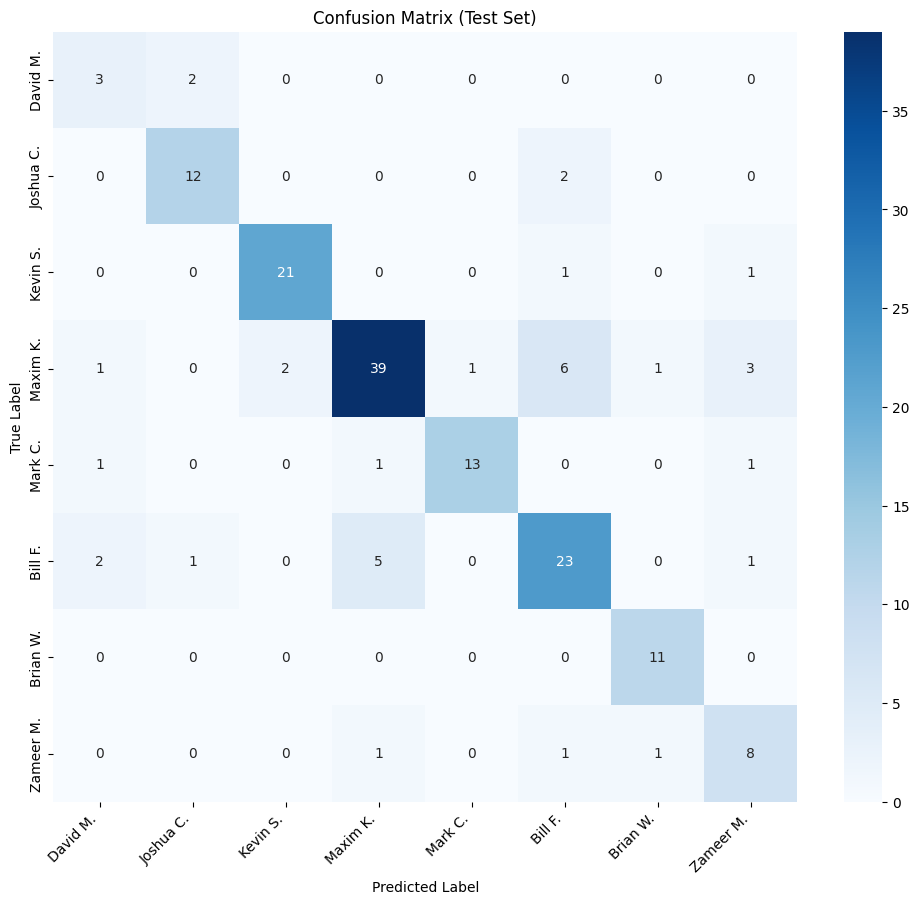
\includegraphics[width=0.68\linewidth]{figures/assignee_confusion_matrix.png}
\caption{Confusion matrix of the assignee model (XGBoost).}
\label{fig:cm_assignee}
\end{figure}

\textbf{Discussion:} Cross-validation indicates stable gains from combining structured features with TF--IDF text. The hold-out results are slightly lower than CV estimates, which is expected when simulating deployment. Top-3 accuracy above 94\% supports practical recommendation usage when workload constraints or manual confirmation are applied.

% ---------------------------------------------------------
\subsection{Deadline Prediction Performance}
% ---------------------------------------------------------

Table~\ref{tab:deadline_baseline} reports MAE on the same unseen 8-sprint test set. The selected model achieves MAE $=0.9157$ days and MAPE $=6.84\%$ with $R^2=0.4354$.

\begin{table}[t]
\centering
\caption{Deadline prediction on the same unseen test split (8 sprints).}
\renewcommand{\arraystretch}{1.08}
\begin{tabular}{l c}
\hline
\textbf{Model} & \textbf{MAE (days)} \\
\hline
Mean predictor (baseline) & 1.3417 \\
Linear Regression & 1.1124 \\
Random Forest (selected) & \textbf{0.9157} \\
\hline
\end{tabular}
\label{tab:deadline_baseline}
\end{table}

\begin{figure}[t]
\centering
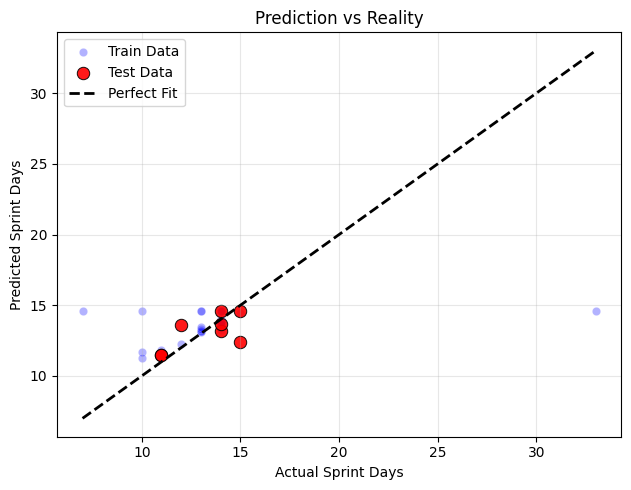
\includegraphics[width=0.75\linewidth]{figures/deadline_scatter.png}
\caption{Predicted vs. actual completion time (days) on the test sprints.}
\label{fig:scatter_deadline}
\end{figure}

\textbf{Discussion:} The selected model reduces MAE by 17.7\% compared to linear regression (1.1124 $\rightarrow$ 0.9157 days) and by 31.8\% compared to the mean baseline (1.3417 $\rightarrow$ 0.9157 days). The moderate $R^2$ suggests substantial unexplained variance driven by latent sprint-time factors not present in the compact feature set. Therefore, predictions should be interpreted as decision support for due-date suggestion, not deterministic forecasts.

% ---------------------------------------------------------
\subsection{Workflow-Level Implications}
% ---------------------------------------------------------

Integration into n8n enables (i) automated completeness enforcement (assignee/due date), (ii) periodic re-evaluation for incomplete or returned issues, and (iii) PR-driven transitions to review/testing with notifications. In practice, end-to-end throughput is dominated by external API calls rather than model inference; model latency remained sub-second per request in local deployment, which is sufficient for asynchronous automation.

% =========================================================
\section{Conclusion}
% =========================================================

This work demonstrates the feasibility of embedding ML inference into an automated Agile workflow for task assignment and deadline estimation. The assignee model achieves 78.79\% Top-1 and 94.55\% Top-3 accuracy on unseen data, indicating that combining lightweight text features with structured metadata supports practical recommendation-based assignment. For deadline prediction, the selected model achieves low absolute error (MAE 0.9157 days, MAPE 6.84\%) on unseen sprints, though explained variance is modest ($R^2=0.435$), reflecting inherent uncertainty in Agile completion time.

The primary contribution is the workflow-aware operationalization: REST-deployed predictors embedded into n8n orchestration with scheduled re-checks and PR-driven transitions. Future work includes incorporating additional process signals available during sprint execution (e.g., PR activity and review duration) and evaluating generalization on larger or proprietary datasets.

% =========================================================
% REFERENCES (chronological / logical order)
% =========================================================

\begin{thebibliography}{00}

% --- References Cited in Introduction (1-11) ---

\bibitem{verwijs2023_scrum}
C. Verwijs and D. Russo, ``A Theory of Scrum Team Effectiveness,''
\textit{ACM Trans. Softw. Eng. Methodol.}, vol. 32, no. 3, Art. 74, Apr. 2023,
doi: 10.1145/3571849.

\bibitem{gemino2021_project_success}
A. Gemino, B. H. Reich, and R. Serrador, ``Agile, traditional, and hybrid approaches to project success: Is hybrid a poor second choice?''
\textit{Project Management Journal}, vol. 52, no. 2, pp. 161--175, 2021,
doi: 10.1177/8756972820973082.

\bibitem{gibbs2023_wfh_productivity}
M. Gibbs, F. Mengel, and C. Siemroth, ``Work from Home and Productivity: Evidence from Personnel and Analytics Data on IT Professionals,''
\textit{J. Political Economy Microeconomics}, vol. 1, no. 2, pp. 235--275, 2023,
doi: 10.1086/721803.

\bibitem{venkatesh2020_work_exhaustion}
V. Venkatesh, J. Y. L. Thong, and F. K. Y. Chan, ``How Agile Software Development Methods Reduce Work Exhaustion: Insights on Role Perceptions and Organizational Skills,''
\textit{Information Systems Journal}, vol. 30, no. 5, pp. 829--859, 2020,
doi: 10.1111/isj.12282.

\bibitem{prinz2021_lowcode_slr}
N. Prinz, C. Rentrop, and M. Huber, ``Low-Code Development Platforms -- A Literature Review,''
in \textit{Proc. Americas Conf. Inf. Syst. (AMCIS)}, 2021.

\bibitem{zhao2021_trigger_action}
D. Zhao \textit{et al.}, ``What Can We Learn from a Dataset of If-This-Then-That Recipes?''
in \textit{Proc. CHI Conf. Human Factors in Computing Systems (CHI)}, 2021,
doi: 10.1145/3411764.3445567.

\bibitem{diamantopoulos2023_issue_assignment}
T. Diamantopoulos, N. Saoulidis, and A. Symeonidis,
``Automated Issue Assignment Using Topic Modelling on Jira Issue Tracking Data,''
\textit{IET Software}, vol. 17, no. 3, pp. 333--344, 2023,
doi: 10.1049/sfw2.12129.

\bibitem{sousa2023_task_effort}
T. Sousa \textit{et al.}, ``Applying Machine Learning to Estimate the Effort and Duration of Individual Tasks in Software Projects,''
\textit{IEEE Access}, vol. 11, pp. 89933--89946, 2023,
doi: 10.1109/ACCESS.2023.3287537.

\bibitem{mahdi2021_spm_slr}
N. Mahdi \textit{et al.}, ``Machine Learning for Software Project Management: A Systematic Literature Review,''
\textit{Applied Sciences}, vol. 11, no. 23, 2021.

\bibitem{cabral2023_ensemble_effort}
J. T. H. d. A. Cabral, R. Gomes, and A. Mendes-Moreira,
``Ensemble Effort Estimation: An Updated and Extended Systematic Literature Review,''
\textit{J. Syst. Softw.}, vol. 195, Art. 111542, 2023,
doi: 10.1016/j.jss.2022.111542.

\bibitem{yasmin2024_airflow_wac}
J. Yasmin, J. Wang, Y. Tian, and B. Adams, ``An Empirical Study of Developers' Challenges in Implementing Workflows as Code: A Case Study on Apache Airflow,''
\textit{arXiv preprint} arXiv:2406.00180, 2024.

% --- References Cited in Related Work (12-19) ---

\bibitem{shamim2025_costreview}
M. M. I. Shamim \textit{et al.},
``Advancement of Artificial Intelligence in Cost Estimation for Project Management Success: A Systematic Review,''
\textit{Modelling}, vol. 6, no. 2, Art. 35, 2025,
doi: 10.3390/modelling6020035.

\bibitem{gupta2023_action_suggestions}
S. Gupta \textit{et al.}, ``Personalized Action Suggestions in Low-Code Automation Platforms,''
in \textit{Proc. IEEE/ACM Int. Conf. Softw. Eng. Companion (ICSE-Companion)}, 2023,
doi: 10.1109/ICSE-Companion58688.2023.00100.

\bibitem{perezcastillo2024_sprint_velocity}
Y. J. P\'erez Castillo, S. D. Orantes Jim\'enez, and P. O. Letelier Torres,
``Sprint Management in Agile Approach: Progress and Velocity Evaluation Applying Machine Learning,''
\textit{Information}, vol. 15, no. 11, Art. 726, 2024,
doi: 10.3390/info15110726.

\bibitem{choetkiertikul2025_sprint2vec}
M. Choetkiertikul \textit{et al.},
``Sprint2Vec: A Deep Characterization of Sprints in Iterative Software Development,''
\textit{IEEE Trans. Softw. Eng.}, vol. 51, no. 1, pp. 220--242, 2025,
doi: 10.1109/TSE.2024.3509016.

\bibitem{ramessur2021_sprint_effort}
S. Ramessur and S. D. Nagowah,
``Software Effort Estimation in a Sprint Using Machine Learning Regression Techniques,''
\textit{Int. J. Inf. Technol.}, vol. 13, pp. 1--10, 2021,
doi: 10.1007/s41870-021-00669-z.

\bibitem{yalciner2024_storypoint_sbert}
B. Yal\c{c}{\i}ner and D. Baturay,
``Enhancing Agile Story Point Estimation: Integrating Deep Learning, Machine Learning, and Natural Language Processing with SBERT and Gradient Boosted Trees,''
\textit{Applied Sciences}, vol. 14, no. 16, Art. 7305, 2024,
doi: 10.3390/app14167305.

\bibitem{guo2020_bug_triage}
S. Guo \textit{et al.}, ``Developer Activity Motivated Bug Triaging: Via Convolutional Neural Network,''
\textit{Neural Process. Lett.}, vol. 52, pp. 1--18, 2020,
doi: 10.1007/s11063-020-10213-y.

\bibitem{zhang2023_susrec}
W. Zhang, J. Zhao, R. Peng, S. Wang, and Y. Yang,
``SusRec: An Approach to Sustainable Developer Recommendation for Bug Resolution Using Multimodal Ensemble Learning,''
\textit{IEEE Trans. Reliability}, vol. 72, no. 1, pp. 61--78, 2023,
doi: 10.1109/TR.2022.3176733.

% --- References Cited Elsewhere / Data / LBE (20-26) ---

\bibitem{mahmud2022_risk_slr}
M. S. Mahmud \textit{et al.}, ``Software Project Risk Prediction Using Machine Learning: A Systematic Literature Review,''
\textit{Applied Sciences}, vol. 12, no. 4, 2022.

\bibitem{nastos2025_resolution_time}
D.-N. Nastos, T. Diamantopoulos, D. Tosi, M. Tropeano, and A. Symeonidis,
``Towards an Interpretable Analysis for Estimating the Resolution Time of Software Issues,''
\textit{arXiv preprint} arXiv:2505.01108, 2025.

\bibitem{brar2022_effort_slr}
A. Brar and A. Nandal,
``A Systematic Literature Review on Software Effort Estimation Using Machine Learning Techniques,''
in \textit{Proc. (IEEE-indexed) Conf.}, 2022.

\bibitem{koralage2023_velocity}
R. U. Koralage, ``Novel Approach to Estimate Velocity for Agile Scrum Sprint Planning,''
Preprint, Dec. 2023.

\bibitem{lbe_9234227}
R. S. Dewi and R. Sarno, ``Software Effort Estimation Using Early COSMIC to Substitute Use Case Weight,''
in \textit{Proc. 2020 International Seminar on Application for Technology of Information and Communication (iSemantic)},
pp. 214--219, 2020, doi: 10.1109/iSemantic50169.2020.9234227.

\bibitem{lbe_11229547}
K. C. Febryanto, S. C. Hidayati, and R. Sarno, ``Multi-Dimensional Quality Assessment of Synthetic Data across ERP Modules,''
in \textit{Proc. 2025 IEEE International Conference on Artificial Intelligence and Mechatronics Systems (AIMS)},
pp. 1--6, 2025, doi: 10.1109/AIMS66189.2025.11229547.

\bibitem{lbe_11019730}
Z. L. Putra, R. Sarno, A. F. Septiyanto, R. Januar Akbar, and F. Taufany,
``Evaluating The Modularity of Domain-Driven Design Approach: A Case Study of Academic Information System,''
in \textit{Proc. 2025 International Conference on Computer Sciences, Engineering, and Technology Innovation (ICoCSETI)},
pp. 507--512, 2025, doi: 10.1109/ICoCSETI63724.2025.11019730.

\end{thebibliography}

\end{document}
